% !TeX root = ../main.tex
\section{FedPASA}
\label{sec:method}

\subsection{Problem Setup and Overview}
\label{sec:setup}

We consider cross-domain federated recommendation with disjoint item catalogs. Let $\mathcal{C}$, $\mathcal{U}$, and $\mathcal{I}$ denote the sets of clients, users, and target items, respectively. Each client $c$ maintains a subset of users $\mathcal{U}_c$ and their interaction histories locally. A frozen text encoder maps each item $i$ to a unit-normalized semantic representation $x_i\in\mathbb{R}^d$, providing a common representation space across domains. Each user $u$ is associated with a private embedding $e_u\in\mathbb{R}^d$ that remains on its corresponding client.

FedPASA adapts the frozen semantic representations through three mechanisms: Popularity-Gated Dual-path Routing (PGDR), Private-Profile Client Conditioning, and Catalog-Level Semantic Anchoring (AutoAnchor). Source-domain training initializes one residual adaptation path, while the second path is randomly initialized on the target domain. Both paths remain trainable during target-domain federated optimization.

For user $u$ on client $c$, the recommendation score is defined as
\begin{equation}
    s(u,i)=e_u^{\top}z^{\mathrm{anchor}}_{c,i}.
    \label{eq:score}
\end{equation}
The model is optimized using Bayesian Personalized Ranking (BPR)~\citep{rendle2009bpr}:
\[
\mathcal{L}_{\mathrm{BPR}}=-\mathbb{E}_{(u,i,j)}\log\sigma\big(\tau[s(u,i)-s(u,j)]\big),
\]
where $i$ is an observed positive item, $j$ a sampled negative item, and $\tau$ controls the score scale.

Figure~\ref{fig:framework} illustrates the overall FedPASA framework, and Table~\ref{tab:notation} summarizes the notation. The forward computation consists of three consecutive stages:
\begin{equation}
x_i \xrightarrow{\mathrm{routing}} h_i
\xrightarrow{\substack{\mathrm{FiLM}\\\mathrm{and\ residual}}} z_{c,i}
\xrightarrow{\mathrm{anchoring}} z^{\mathrm{anchor}}_{c,i}.
\label{eq:pipeline}
\end{equation}

\begin{figure*}[t]
\centering
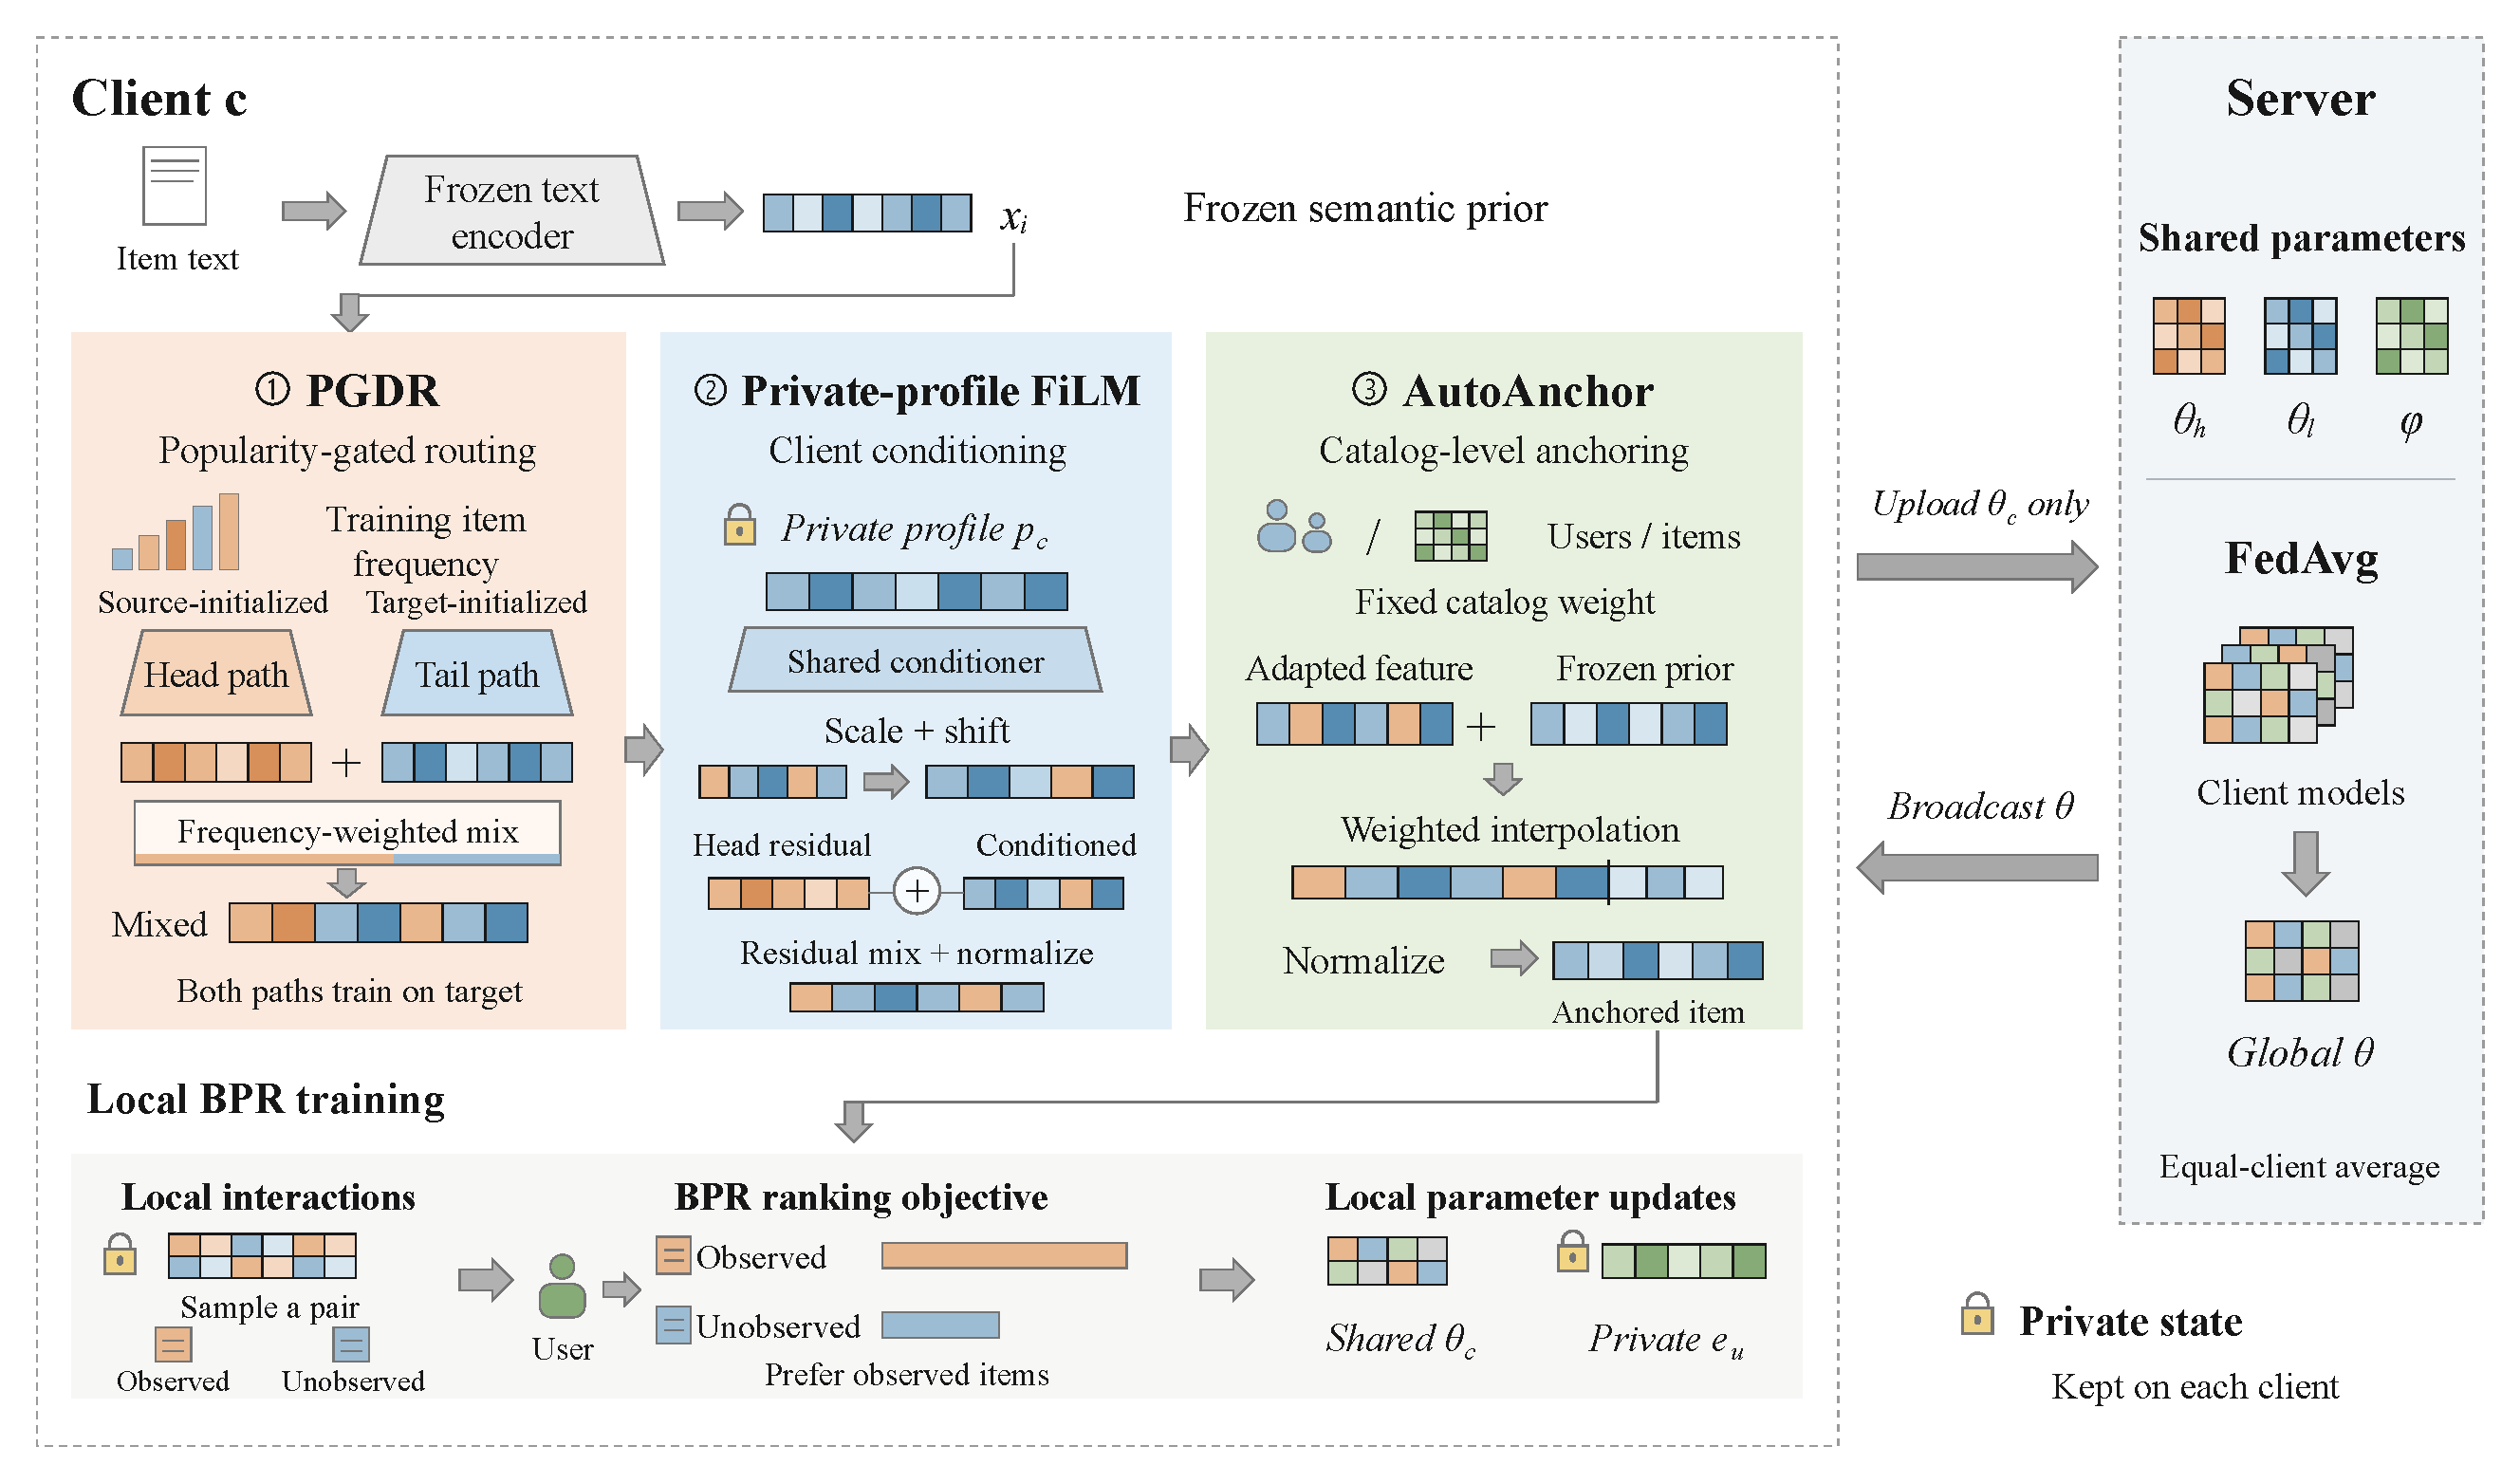
\includegraphics[width=\textwidth]{figures/FedPASA_framework_graphic.pdf}
\caption{FedPASA framework. PGDR combines source-initialized and target-initialized residual adapters according to item frequency. Private-profile FiLM conditions the resulting representations on local interaction semantics, while AutoAnchor integrates the frozen semantic prior. Clients optimize shared model parameters and private user embeddings using BPR, and the server aggregates the shared parameters through FedAvg.}
\label{fig:framework}
\end{figure*}

\subsection{Popularity-Gated Dual-path Routing}
\label{sec:pgdr}

Target items exhibit substantially different interaction frequencies, resulting in different amounts of supervision for semantic adaptation. PGDR explicitly uses item frequency to determine the relative contributions of two residual adaptation paths, enabling frequency-dependent representation learning within a shared model.

Let $\mathrm{freq}(i)$ denote the number of target-domain training interactions containing item $i$. We first construct an inverse-frequency score $\bar q_i=1/\sqrt{\mathrm{freq}(i)+1}$ and normalize it over the target catalog:
\begin{equation}
q_i=\frac{\bar q_i-\min_j \bar q_j}{\max_j \bar q_j-\min_j \bar q_j+\epsilon}.
\label{eq:coldness}
\end{equation}
A threshold $t$ and exponent $\kappa$ further reshape the routing score:
\[
q_i'=\mathrm{clip}\!\big(\tfrac{q_i-t}{1-t},0,1\big)^{\kappa}.
\]
The resulting score $q_i'$ increases as item frequency decreases and controls the relative contribution of the target-initialized path.

PGDR contains two residual adapters, denoted by $A_h$ and $A_l$. The head adapter $A_h$ is initialized from the source-domain adapter, providing transferred semantic adaptation knowledge. The tail adapter $A_l$ is randomly initialized on the target domain and learns complementary transformations from target interactions. Each adapter contains two sequential residual blocks, $v\leftarrow v+F_\ell(v)$, where $F_\ell$ is a bottleneck multilayer perceptron, followed by $\ell_2$ normalization. Both adapters are optimized during target-domain federated training.

The routed item representation is
\begin{equation}
h_i=(1-q_i')\,A_h(x_i)+q_i'\,A_l(x_i).
\label{eq:routing}
\end{equation}
Frequently observed items place greater weight on the source-initialized head path, whereas lower-frequency items receive a larger contribution from the target-initialized tail path. The mixed representation $h_i$ is subsequently passed to the client-conditioning module.

\subsection{Private-Profile Client Conditioning}
\label{sec:conditioning}

Item frequency characterizes supervision at the item level, while clients may observe substantially different semantic regions of the target catalog. To incorporate this client-side heterogeneity, FedPASA constructs a private semantic profile from each client's local interaction history and uses it to condition the routed representation.

For client $c$, let $\mathcal{I}_c$ denote the multiset of items appearing in its training interactions. Repeated interactions retain their multiplicity in the profile construction. The client profile is defined as
\begin{equation}
p_c=\mathrm{norm}\Big(\tfrac{1}{|\mathcal{I}_c|}\sum_{i\in\mathcal{I}_c} x_i\Big).
\label{eq:profile}
\end{equation}
A shared bottleneck network $g_\phi:\mathbb{R}^d\!\to\!\mathbb{R}^{2d}$ maps the profile into feature-wise FiLM parameters:
\begin{equation}
(\gamma_c,\beta_c)=g_\phi(p_c).
\label{eq:filmparams}
\end{equation}
The routed representation $h_i$ is then modulated as
\begin{equation}
\begin{aligned}
m_{c,i}&=h_i\odot(1+\lambda\,\tanh\gamma_c)+\lambda\beta_c,\\
z_{c,i}&=\mathrm{norm}\big((1-\alpha)A_h(x_i)+\alpha m_{c,i}\big).
\end{aligned}
\label{eq:film}
\end{equation}
The coefficient $\lambda$ controls the strength of client-dependent modulation. The $\tanh$ transformation bounds the multiplicative factor to $[1-\lambda,1+\lambda]$, while the additive term provides learned client-specific feature shifts. The coefficient $\alpha\in[0,1]$ controls the contribution of the conditioned representation relative to the head-path residual.

For the conditioning module, only the shared parameters $\phi$ participate in federated communication. The client profile $p_c$ is computed from local training interactions and remains on the client.

\subsection{Catalog-Level Semantic Anchoring}
\label{sec:anchor}

After frequency-aware routing and client conditioning, FedPASA further integrates the frozen semantic representation into the final ranking representation. AutoAnchor determines the contribution of this semantic prior according to target-catalog coverage.

We characterize target-catalog coverage using the user-to-item ratio
\[
\eta_T=|\mathcal{U}_T|/|\mathcal{I}_T|,
\]
where $|\mathcal{U}_T|$ denotes the number of observed target-domain users and $|\mathcal{I}_T|$ denotes the target catalog size. Given coverage thresholds $\tau_l<\tau_h$ and maximum anchor weight $\rho$, AutoAnchor computes
\begin{equation}
\begin{aligned}
\rho_{\mathrm{eff}}&=\rho\cdot\mathrm{clip}\!\Big(\frac{\tau_h-\eta_T}{\tau_h-\tau_l},0,1\Big),\\
z^{\mathrm{anchor}}_{c,i}&=\mathrm{norm}\big((1-\rho_{\mathrm{eff}})\,z_{c,i}+\rho_{\mathrm{eff}}\,x_i\big).
\end{aligned}
\label{eq:anchor}
\end{equation}
The effective weight $\rho_{\mathrm{eff}}$ controls the contribution of the frozen semantic prior. When $\eta_T\leq\tau_l$, the maximum anchor weight $\rho$ is used. As $\eta_T$ increases between $\tau_l$ and $\tau_h$, the prior contribution decreases linearly. For $\eta_T\geq\tau_h$, the final representation relies directly on the adapted representation. Its weight is determined from target-domain catalog statistics and remains fixed throughout federated training and evaluation.

The default catalog-level gate introduces no additional trainable parameters. We additionally evaluate a per-item learnable alternative,
\[
\rho_i=\rho\,\sigma(a_i),
\]
where $a\in\mathbb{R}^{|\mathcal{I}|}$ contains item-specific logits included in federated aggregation. The corresponding comparison is reported in the anchor analysis (\S\ref{sec:exp-anchor}).

\subsection{Federated Training and Local Personalization}
\label{sec:training}

FedPASA jointly learns shared semantic adaptation parameters across clients while maintaining private user representations locally. The shared trainable parameters are $\theta=\{\theta_h,\theta_l,\phi\}$, where $\theta_h$ and $\theta_l$ denote the parameters of the two residual adapters and $\phi$ denotes the parameters of the client-conditioning network. Each client $c$ additionally maintains a private user-embedding table $E_c=\{e_u:u\in\mathcal{U}_c\}$.

During communication round $r$, the server broadcasts the current shared parameters $\theta^{(r)}$ to all participating clients. Each client initializes its local shared-model copy from $\theta^{(r)}$, retains its private user embeddings from the preceding round, and performs $K$ local optimization steps using the BPR objective. The local optimization updates both the shared parameters $\theta_c$ and private user embeddings $E_c$. After local training, each client uploads only $\theta_c$ to the server. Under the default full-participation setting, the server performs equal-client FedAvg:
\[
\theta^{(r+1)}=\frac{1}{|\mathcal{C}|}\sum_{c\in\mathcal{C}}\theta_c.
\]
The federated adaptation stage optimizes the BPR objective without an additional proximal penalty.

After $R$ communication rounds, the resulting global parameters $\theta^{(R)}$ define the shared FedPASA model. We refer to this model before final local personalization as \emph{FedPASA base}. For final personalization, each client initializes its local model from $\theta^{(R)}$, retains its learned private user embeddings, and optimizes
\[
\mathcal{L}_{\mathrm{pers},c}
=
\mathcal{L}_{\mathrm{BPR},c}
+
\frac{\mu_p}{2}\,\|\theta_c-\theta^{(R)}\|_2^2.
\]
The proximal term encourages local adaptation around the final global solution~\citep{li2020federated,li2021ditto}. During this stage, both $\theta_c$ and $E_c$ are updated, while the proximal penalty is applied only to the shared-model parameters $\theta_c$. Each client performs $K_p$ local personalization steps. The resulting personalized parameters remain local and are not uploaded to the server.

Algorithm~\ref{alg:training} summarizes the complete training procedure. Concrete optimization settings are provided in the experimental setup (\S\ref{sec:exp-setup}).

\begin{algorithm}[t]
\caption{FedPASA training and local personalization}
\label{alg:training}
\footnotesize
\begin{algorithmic}[1]
\Require Frozen item features, training histories, clients $\mathcal{C}$, rounds $R$, local steps $K$, personalization steps $K_p$, proximal coefficient $\mu_p$
\State For cross-domain training, optimize a source-domain residual adapter by source BPR and equal-client FedAvg
\State Initialize $\theta_h$ from the source adapter; randomly initialize $\theta_l$ and $\phi$
\State Compute target routing scores $q_i$ from target training frequencies
\State Compute each client profile $p_c$ from its training interactions
\State Compute and fix the catalog-level anchor weight $\rho_{\mathrm{eff}}$
\State Initialize private user tables $E_c=\{e_u:u\in\mathcal{U}_c\}$ for all clients
\State $\theta^{(0)}\gets\{\theta_h,\theta_l,\phi\}$
\For{$r=0,\ldots,R-1$}
    \State Broadcast $\theta^{(r)}$ to all participating clients
    \ForAll{$c\in\mathcal{C}$ \textbf{in parallel}}
        \State $\theta_c\gets\theta^{(r)}$; retain $E_c$ from the preceding round
        \State Take $K$ local steps on $\mathcal{L}_{\mathrm{BPR}}$, updating $(\theta_c,E_c)$
        \State Keep $E_c$ local and upload $\theta_c$
    \EndFor
    \State $\theta^{(r+1)}\gets |\mathcal{C}|^{-1}\sum_{c\in\mathcal{C}}\theta_c$
\EndFor
\State Preserve $\theta^{(R)}$ as the FedPASA base model
\ForAll{$c\in\mathcal{C}$}
    \State $\theta_c\gets\theta^{(R)}$; retain the final $E_c$
    \State $\ell_c\gets\mathcal{L}_{\mathrm{BPR}}+\frac{\mu_p}{2}\|\theta_c-\theta^{(R)}\|_2^2$
    \State Take $K_p$ local personalization steps, updating $(\theta_c,E_c)$
\EndFor
\State \Return Personalized $(\theta_c,E_c)$ stored on each client
\end{algorithmic}
\end{algorithm}

\paragraph{Initialization and local optimization.}
Source-domain training uses one residual adapter together with source-domain user embeddings. The resulting adapter parameters initialize the target-domain head path. The tail path is randomly initialized. The final linear layer of the conditioning network is zero-initialized so that client modulation starts from the shared representation.

Target item frequencies are computed exclusively from target training interactions. Each client profile is computed from its own training-item multiset, with repeated interactions retained. Routing statistics, client profiles, and the catalog-level anchor weight are fixed throughout federated optimization, personalization, and evaluation.

Private user embeddings persist across communication rounds. AdamW optimizer states are reset at the beginning of each local optimization phase. During local training, users are sampled uniformly within a client and positive items are sampled uniformly from the corresponding user's training history. Negative items are sampled from items outside the user's observed training interactions. Dropout is enabled during model updates and disabled during evaluation.

The communication process exchanges only the shared adaptation and conditioning parameters. Raw interaction histories, client profiles, and private user embeddings remain on their respective clients.

\subsection{Analysis of the Adaptation Controls}
\label{sec:theory}

We analyze the main adaptation mechanisms from three perspectives: the relationship between target-estimation reliability and semantic-prior weighting, the geometry of normalized semantic anchoring, and the interaction between popularity routing and client conditioning.

\subsubsection{Bias--Variance Tradeoff of Prior Weighting}

\begin{proposition}[Bias--variance tradeoff]
\label{thm:anchor}
Let $z^*$ denote an ideal target representation and $x$ a semantic prior. Consider an estimated target representation $\hat z=z^*+\varepsilon$, where $\mathbb{E}\varepsilon=0$ and $\mathbb{E}\|\varepsilon\|_2^2=\sigma^2/r$ with $r,\sigma^2>0$. Here, $r$ characterizes the reliability of the target estimate: larger $r$ corresponds to lower estimation variance. Let $b^2=\|x-z^*\|_2^2$ denote the squared bias of the semantic prior. For the interpolated estimate $\tilde z_\omega=(1-\omega)\hat z+\omega x$, we have
\begin{equation}
\mathbb{E}\|\tilde z_\omega-z^*\|_2^2
=(1-\omega)^2\sigma^2/r+\omega^2b^2,
\qquad
\omega^*=\frac{\sigma^2}{\sigma^2+rb^2}.
\label{eq:biasvar}
\end{equation}
When $b>0$, $\omega^*$ decreases as $r$ increases.
\end{proposition}

The optimal weight increases with estimation noise and decreases with prior bias: when target evidence is limited, more of a useful prior should be retained. AutoAnchor operationalizes this principle at the catalog level by using target-catalog coverage to determine the contribution of the frozen semantic prior.

\subsubsection{Geometry of Normalized Semantic Anchoring}

\begin{proposition}[Normalized anchor geometry]
\label{thm:drift}
For fixed unit vectors $x$ and $z$, define $w_\omega=(1-\omega)z+\omega x$, $y_\omega=w_\omega/\|w_\omega\|_2$, and $a=x^\top z$. For $0\le\omega<1/2$,
\begin{equation}
\|w_\omega\|_2\ge1-2\omega>0,
\qquad
\frac{d(x^\top y_\omega)}{d\omega}
=\frac{(1-\omega)(1-a^2)}{\|w_\omega\|_2^3}\ge0.
\label{eq:drift}
\end{equation}
Therefore, $1-x^\top y_\omega$ is non-increasing with respect to the anchor weight $\omega$.
\end{proposition}

This proposition characterizes the geometric effect of normalized semantic interpolation: for a fixed adapted representation, increasing the anchor weight moves the final representation toward the frozen semantic prior. The experimental analysis (\S\ref{sec:exp-drift}) further examines the representation geometry produced after federated optimization.

\subsubsection{Client Conditioning}

The multiplicative part of the FiLM transformation in Eq.~\eqref{eq:film} is $1+\lambda\tanh\gamma_c$. Since $\tanh\gamma_c\in[-1,1]$, the resulting feature-wise multiplicative factors satisfy $1-\lambda\le1+\lambda\tanh\gamma_c\le1+\lambda$. Thus, $\lambda$ directly controls the range of client-dependent multiplicative modulation, while the learned additive term $\lambda\beta_c$ shifts the routed representation according to the client's semantic profile.

\subsubsection{Interaction of Routing and Client Conditioning}

PGDR and client conditioning act on the same semantic representation but control different aspects of adaptation. To make the interaction explicit, consider the case in which FiLM modulation is disabled, i.e., $\lambda=0$. Combining Eqs.~\eqref{eq:routing} and~\eqref{eq:film} gives
\begin{equation}
z_{c,i}=\mathrm{norm}\big((1-\alpha q_i')A_h(x_i)+\alpha q_i'A_l(x_i)\big).
\label{eq:effective-routing}
\end{equation}
The effective coefficient of the target-initialized path is therefore $\alpha q_i'$. The item-frequency-derived score $q_i'$ determines how the two adaptation paths are allocated to each item, while $\alpha$ controls the overall strength of this allocation. Even for the largest routing score $q_i'=1$, the head path retains a contribution of $1-\alpha$.

When FiLM is enabled, client-dependent feature scales and shifts are applied to the frequency-routed representation before normalization and semantic anchoring. Consequently, item frequency controls path combination, whereas the private client profile controls feature-level adjustment.


